\documentclass[a4paper, 11pt]{article}

\usepackage{geometry}
\usepackage{amsmath,amssymb}
\usepackage{ifthen}
\usepackage{subcaption}
\usepackage{booktabs}
\usepackage{siunitx}
\usepackage[section]{placeins}

\usepackage{tikz}
\usetikzlibrary{calc,math}

\makeatletter
\pgfdeclareshape{oplus}{%{{{
  \inheritsavedanchors[from=circle]
  \inheritanchorborder[from=circle]
  \foreach \s in {center,mid,base,text, north,south,west,east,
                  mid west,mid east,base west,base east,
                  north west,south west,north east,south east} {
    \inheritanchor[from=circle]{\s}
  }
  \backgroundpath{%
    \pgfutil@tempdima=\radius%
    \pgfmathsetlength{\pgf@xb}{\pgfkeysvalueof{/pgf/outer xsep}}%  
    \pgfmathsetlength{\pgf@yb}{\pgfkeysvalueof{/pgf/outer ysep}}%  
    \ifdim\pgf@xb<\pgf@yb%
      \advance\pgfutil@tempdima by-\pgf@yb%
    \else%
      \advance\pgfutil@tempdima by-\pgf@xb%
    \fi%
    \pgfpathcircle{\centerpoint}{\pgfutil@tempdima}%
    % north-south
    \centerpoint\advance\pgf@y by\radius  \pgf@xa=\pgf@x \pgf@ya=\pgf@y
    \centerpoint\advance\pgf@y by-\radius \pgf@xb=\pgf@x \pgf@yb=\pgf@y
    \pgfpathmoveto{\pgfpoint{\pgf@xa}{\pgf@ya}}
    \pgfpathlineto{\pgfpoint{\pgf@xb}{\pgf@yb}}
    % east-west
    \centerpoint\advance\pgf@x by\radius  \pgf@xa=\pgf@x \pgf@ya=\pgf@y
    \centerpoint\advance\pgf@x by-\radius \pgf@xb=\pgf@x \pgf@yb=\pgf@y
    \pgfpathmoveto{\pgfpoint{\pgf@xa}{\pgf@ya}}
    \pgfpathlineto{\pgfpoint{\pgf@xb}{\pgf@yb}}
  }
}%}}}
\makeatother
\tikzset{op/.style={draw, fill=none, minimum size=1.25ex, inner sep=0pt}}
\tikzset{opxor/.style={op, shape=oplus}}
\tikzset{opand/.style={op, rectangle, rounded corners=2pt, minimum height=3ex}}
\tikzset{oprot/.style={op, rectangle, rounded corners=2pt, inner sep=2pt, minimum width=3ex, font=\scriptsize}}
\tikzset{optee/.style={shape=circle, fill, draw, inner sep=0pt, minimum size=2pt}}
\tikzset{next/.style={->, >=latex}}
\tikzset{trail/.style={line width=2pt, line cap=round}}
\definecolor{delta}{HTML}{B58900}
\definecolor{epsil}{HTML}{CB4B16}
\definecolor{gamma}{HTML}{6C71C4}
\definecolor{beta}{HTML}{268BD2}
\definecolor{alpha}{HTML}{859900}

%\definecolor{mybase0}{HTML}{839496}
%\definecolor{mybase1}{HTML}{93A1A1}
%\definecolor{mybase2}{HTML}{EEE8D5}
%\definecolor{mybase3}{HTML}{FDF6E3}
%\definecolor{myred}{HTML}{DC322F}
%\definecolor{mymagenta}{HTML}{D33682}
%\definecolor{mycyan}{HTML}{2AA198}

\newcommand{\cipher}[1]{\textsf{#1}}

\newif\ifsubstates\substatesfalse

\newcommand{\printstate}{
  \ifsubstates \pgfmathsetmacro{\roundsep}{1.25}
  \else        \pgfmathsetmacro{\roundsep}{0.80} \fi
  \pgfmathsetmacro{\opoffset}{.1}

  \ifsubstates
    \foreach \r in {-2,...,4} {
      \foreach \w in {0,...,4} {
        \draw[thick] (\w-.5,-\r*\roundsep) -- ++(0,-.25);
        \node[minimum width=1*1.0cm,minimum height=.25*1.5cm, inner sep=0pt] (W\r\w) at (\w,-\r*\roundsep-.125) {};
      }
      \draw[thick] (-.5,-\r*\roundsep) node[below left, inner sep=0pt, xshift=-3pt] {$S_{\r,*}^{\r}$} rectangle ++(5,-.25);
    }
    \node[minimum width=1*1.0cm,minimum height=.25*1.5cm, inner sep=0pt] (W-1-1) at (-1,--1*\roundsep-.125) {};
    \node[minimum width=1*1.0cm,minimum height=.25*1.5cm, inner sep=0pt] (W-2-1) at (-2,--1*\roundsep-.125) {};
  \else
    \foreach \r in {-1,...,4} {
      \foreach \w in {0,...,4} {
        \coordinate (W\r\w) at (\w,-\r*\roundsep-.125);
      }
    }
    \foreach \w in {0,...,4} {
      \coordinate (W-2\w) at (\w,--2.375*\roundsep-.125);
    }
    \coordinate (W-1-1) at (-1,--1*\roundsep-.125);
    \coordinate (W-2-1) at (-2,--1*\roundsep-.125);
  \fi

  %\foreach \r/\rot in {-1/0,0/5,1/31,2/7,3/22,4/13} { % round
  \foreach \r/\rot in {-1/0,0/b_0,1/b_1,2/b_2,3/b_3,4/b_4} { % round
    \ifthenelse{\equal{\r}{-1}}{
      \pgfmathsetmacro{\txorx}{int(mod(\r+2,5))}
      \pgfmathsetmacro{\tanAx}{int(mod(\r+4,5))}
      \pgfmathsetmacro{\tanBx}{int(mod(\r+3,5))}
      \pgfmathsetmacro{\tlllx}{int(mod(\r+1,5))}
    }{
      \pgfmathsetmacro{\txorx}{int(mod(\r+3,5))}
      \pgfmathsetmacro{\tanAx}{int(mod(\r+2,5))}
      \pgfmathsetmacro{\tanBx}{int(mod(\r+1,5))}
    }
    \pgfmathsetmacro{\rprev}{int(\r-1)}
    \ifthenelse{\equal{\r}{-1}}%
    { \node[opxor] (lll\r) at ($(W\r\r) +(0,\opoffset+.25)$)  {}; }%
    { \node[oprot] (lll\r) at ($(W\r\r) +(0,\opoffset+.25)$)  {$\lll\!\rot$}; }
      \node[opxor] (xor\r) at ($(W\r\r) +(0,\opoffset+.50)$)  {};
      \node[opxor] (xnd\r) at ($(W\r\r) +(0,\opoffset+.75)$)  {};
    \ifthenelse{\equal{\r}{4}}
    { \node[opand] (and\r) at ($(W\r3) +(.5,\opoffset+.75)$)  {$\cdot$}; }
    { \node[opand] (and\r) at ($(W\r\r) +(.5,\opoffset+.75)$) {$\cdot$}; }
    \ifthenelse{\equal{\r}{-1}}%
    { \node[inner sep=1pt] (M) at ($(xnd\r) +(0,.45)$) {$M$};
      \node[inner sep=1pt] (C) at ($(lll\r) +(0,-.5)$) {$C$};
      \draw[next] (M) -- (xnd\r);
      \draw[next] (lll\r) -- (C);
      \coordinate[optee] (tlll\r) at ($(W\r\tlllx) +(0,\opoffset+.25)$); }{}
      \coordinate[optee] (txor\r) at ($(W\r\txorx) +(0,\opoffset+.50)$);
      \coordinate[optee] (tanA\r) at ($(W\r\tanAx) +(0,\opoffset+.675)$);
      \coordinate[optee] (tanB\r) at ($(W\r\tanBx) +(0,\opoffset+.825)$);

    \ifthenelse{\equal{\r}{-1}}%
    { \draw[next] (tlll\r) -- (lll\r); }{}
      \draw[next] (txor\r) -- (xor\r);
    \ifthenelse{\tanAx < \r}%
    { \draw[next] (tanA\r) -- (tanA\r-|and\r.west); }%
    { \draw[next] (tanA\r) -- (tanA\r-|and\r.east); }
    \ifthenelse{\tanBx < \r}%
    { \draw[next] (tanB\r) -- (tanB\r-|and\r.west); }%
    { \draw[next] (tanB\r) -- (tanB\r-|and\r.east); }
    \draw[next] (and\r) -- (xnd\r);
    \draw[    ] (xnd\r) -- (xor\r);
    \draw[    ] (xor\r) -- (lll\r);

    \foreach \w in {0,...,4} {
      \ifthenelse{\equal{\w}{\r}}{
        \draw (W\rprev\w) -- (xnd\r);
        \draw (lll\r) -- (W\r\w);
      }{
        \draw (W\rprev\w) -- (W\r\w);
      }
    }
  }
}

\begin{document}

\section{Description of \cipher{MORUS} and \cipher{MiniMORUS}}

\begin{figure}[h]
  \substatesfalse
  % \substatesfalse to label state words and/or masks
  \centering
  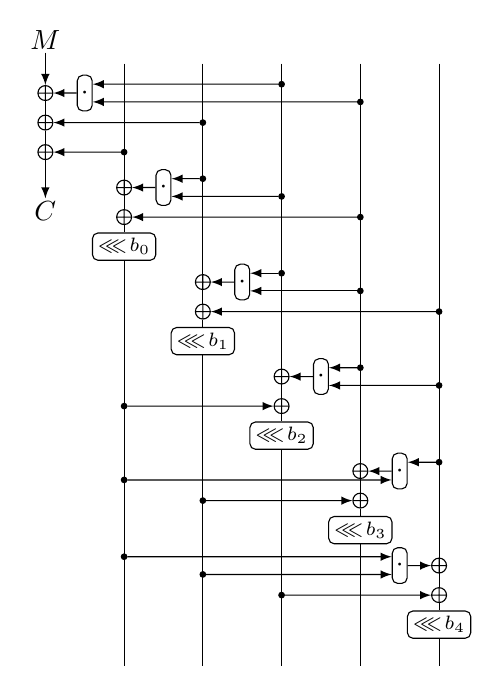
\begin{tikzpicture}[xscale=1.0,yscale=1.5]%{{{
    \printstate
  \end{tikzpicture}%}}}
  \caption{\cipher{MiniMORUS} state update function (1 step = 5 rounds).}
  \label{fig:minimorus}
\end{figure}

\clearpage


\section{Linear Approximations for \cipher{MiniMORUS}}

\noindent
2 approximations for $S^{2,2}_{0}$ of \cipher{MiniMORUS-640}:
\begin{align*}
  S^{2,2}_0 &= C^0_{27} \oplus C^1_{0, 8, 26} \oplus C^2_{7,13,31} \oplus C^3_{12} \tag{corr. $2^{-7}$} \\
  S^{2,2}_0 &= C^1_{2} \oplus C^2_{1,7,15,27} \oplus C^3_{6,14,20} \oplus C^4_{19} \tag{corr. $2^{-9}$} \\
\intertext{Combined ciphertext-only approximation:}
  0 &= C^0_{27} \oplus C^1_{0, 2, 26, 8} \oplus C^2_{1,13,15,27,31} \oplus
  C^3_{6,12,14,20} \oplus C^4_{19} \tag{corr. $\approx 2^{-15.5}$}
\end{align*}
\bigskip

\noindent
2 approximations for $S^{2,2}_{0}$ of \cipher{MiniMORUS-1280}:
\begin{align*}
  S^{2,2}_0 &= C^0_{51} \oplus C^1_{0, 33, 55} \oplus C^2_{4,37,46} \oplus C^3_{50} \tag{corr. $2^{-7}$} \\
  S^{2,2}_0 &= C^1_{25} \oplus C^2_{7,29,38,51} \oplus C^3_{11,20,42} \oplus C^4_{24} \tag{corr. $2^{-9}$} \\
\intertext{Combined ciphertext-only approximation:}
  0 &= C^0_{51} \oplus C^1_{0, 25, 33, 55} \oplus C^2_{4,7,29,37,38,46,51} \oplus C^3_{11,20,42,50} \oplus C^4_{24} \tag{corr. $\approx 2^{-??}$}
\end{align*}


\begin{table}
  \caption{Verification of approximations}
  \begin{tabular}{@{}llSSSS@{}}
    \toprule
    & & \multicolumn{4}{@{}c@{}}{Weight} \\
    \cmidrule{3-6}
    \multicolumn{2}{@{}l}{Approximations for \cipher{MiniMORUS-640}}
             & {Na\"{\i}ve} & {Exp.} & {Bool.} & {Meas.} \\
    \midrule
    $\chi_1$ & $S^{2,2}_0 = C^0_{27} \oplus C^1_{0, 8, 26} \oplus C^2_{7,13,31} \oplus C^3_{12}$
             &            & 7    & 7     & 7 \\
    $\chi_2$ & $S^{2,2}_0 = C^1_{2} \oplus C^2_{1,7,15,27} \oplus C^3_{6,14,20} \oplus C^4_{19}$
             &            & 9    & 9     & 9 \\
    $\chi$   & $0 = C^0_{27} \oplus C^1_{0, 2, 26, 8} \oplus C^2_{1,13,15,27,31} \oplus C^3_{6,12,14,20} \oplus C^4_{19}$
             &            & 16   & 16    & 15.5 \\
    \midrule
    \multicolumn{2}{@{}l}{Approximations for \cipher{MiniMORUS-1280}} \\
    $\chi_1$ & $S^{2,2}_0 = C^0_{51} \oplus C^1_{0, 33, 55} \oplus C^2_{4,37,46} \oplus C^3_{50}$
             &            & 7    & {?}   & 7 \\
    $\chi_2$ & $S^{2,2}_0 = C^1_{25} \oplus C^2_{7,29,38,51} \oplus C^3_{11,20,42} \oplus C^4_{24}$
             &            & 9    & {?}   & 9 \\
    $\chi$   & $0 = C^0_{51} \oplus C^1_{0, 25, 33, 55} \oplus C^2_{4,7,29,37,38,46,51} \oplus C^3_{11,20,42,50} \oplus C^4_{24}$
             &            & 16   & 16    & {??} \\
    \bottomrule
  \end{tabular}
\end{table}


\begin{figure}
  \substatesfalse
  % \substatesfalse to label state words and/or masks
  \centering
  \begin{subfigure}{.32\textwidth}
  \centering
  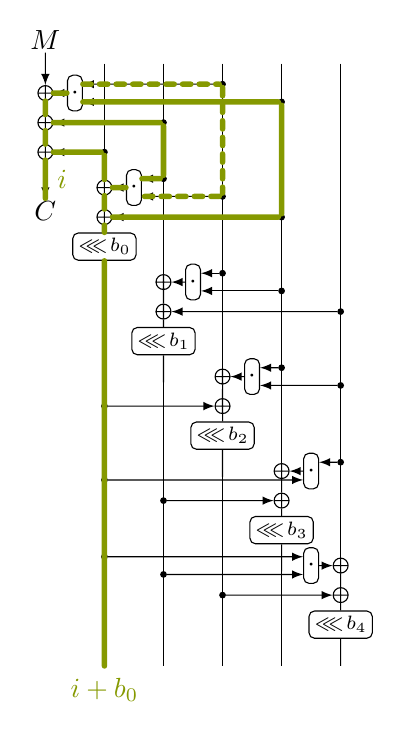
\begin{tikzpicture}[xscale=0.75,yscale=1.5]%{{{
    \printstate
    \draw[trail, alpha]
      (C) -- node[right] {$i$} (lll-1)
      (lll-1) -- (tlll-1) (lll-1) -- (xor-1) (xor-1) -- (xnd-1)
      (xnd-1) -- (and-1) (xor-1) -- (txor-1) (txor-1) -- (tanB0) (tanB0) -- (tanB0-|and0.east)
      (and0) -- (xnd0) (xnd0) -- (tlll-1) (xnd0) -- (xor0)
      (and-1.east|-tanA-1) -- (tanA-1) (tanA-1) -- (txor0) (txor0) -- (xor0)
      (xor0) -- (lll0) (lll0) -- (W40) node[below] {$i+b_0$}
      ;
    \draw[trail, alpha, dashed]
      (and-1.east|-tanB-1) -- (tanB-1) (tanB-1) -- (tanA0) (tanA0) -- (tanA0-|and0.east)
      ;
  \end{tikzpicture}%}}}
  \caption*{$\alpha_i$: weight 1 (not 2)} %$C^j_i, S^{j-1,0}_{i+5}$ ($w\!=\!1$)}
  \end{subfigure}
  \hfill
  \begin{subfigure}{.32\textwidth}
  \centering
  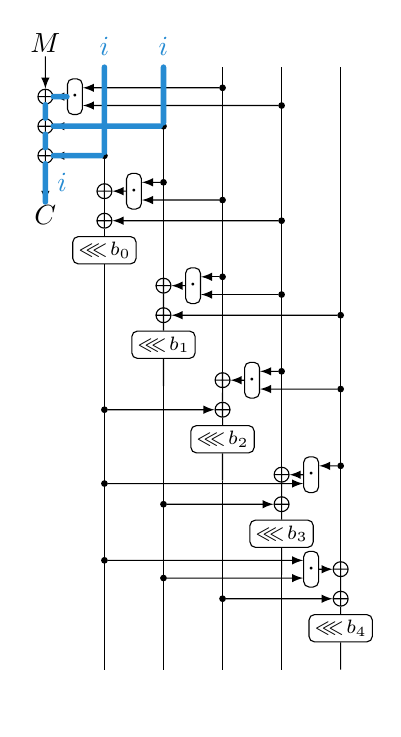
\begin{tikzpicture}[xscale=0.75,yscale=1.5]%{{{
    \printstate
    \draw[trail, beta]
      (C) -- node[right] {$i$} (lll-1)
      (lll-1) -- (tlll-1) (lll-1) -- (xor-1) (xor-1) -- (xnd-1)
      (tlll-1) -- (W-20) node[above] {$i$}
      (xor-1) -- (txor-1) (txor-1) -- (W-21) node[above] {$i$}
      (xnd-1) -- (and-1)
      (W40) node[below] {\phantom{$i$}}
      ;
  \end{tikzpicture}%}}}
  \caption*{$\beta_i$: weight 1} %$C^j_i, S^{j,0}_i, S^{j,1}_i$ ($w\!=\!0$)}
  \end{subfigure}
  \hfill
  \begin{subfigure}{.32\textwidth}
  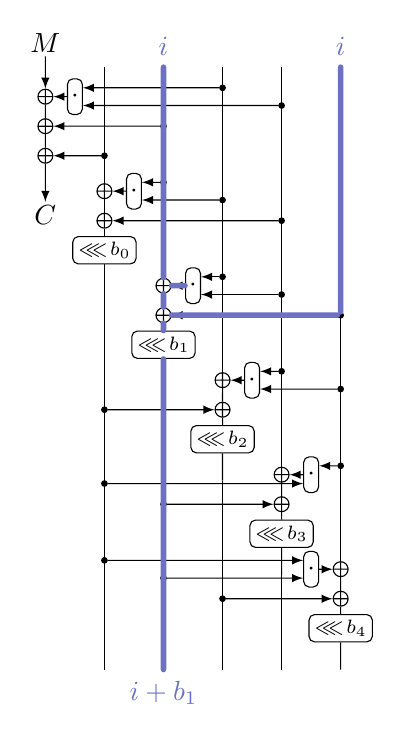
\begin{tikzpicture}[xscale=0.75,yscale=1.5]%{{{
    \printstate
    \draw[trail, gamma]
      (W-21) node[above] {$i$} -- (xnd1) (xnd1) -- (xor1) (xor1) -- (lll1)
      (xnd1) -- (and1)
      (xor1) -- (txor1)
      (txor1) -- (W-24) node[above] {$i$}
      (lll1) -- (W41) node[below] {$i+b_1$}
      ;
  \end{tikzpicture}%}}}
  \caption*{$\gamma_i$: weight 1} %$S^{j,1}_i, S^{j,4}_i, S^{j+1,1}_{i-1}$ ($w\!=\!1$)}
  \end{subfigure}
  \bigskip

  \begin{subfigure}{.32\textwidth}
  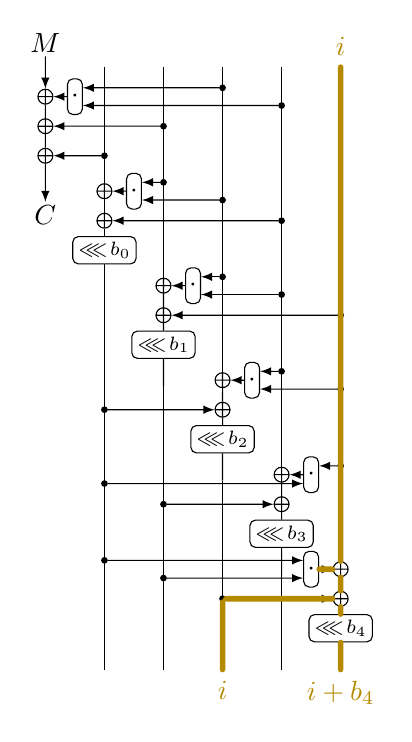
\begin{tikzpicture}[xscale=0.75,yscale=1.5]%{{{
    \printstate
    \draw[trail, delta]
      (W-24) node[above] {$i$} -- (xnd4) (xnd4) -- (xor4) (xnd4) -- (and4)
      (xor4) -- (lll4) (xor4) -- (txor4) (txor4) -- (W42) node[below] {$i$}
      (lll4) -- (W44) node[below] {$i+b_4$}
      ;
  \end{tikzpicture}%}}}
  \caption*{$\delta_i$: weight 1} %$S^{j,4_i}, S^{j+1,2}_i, S^{j+1,4}_{i+13}$ ($w\!=\!1$)}
  \end{subfigure}
  \hfill
  \begin{subfigure}{.32\textwidth}
  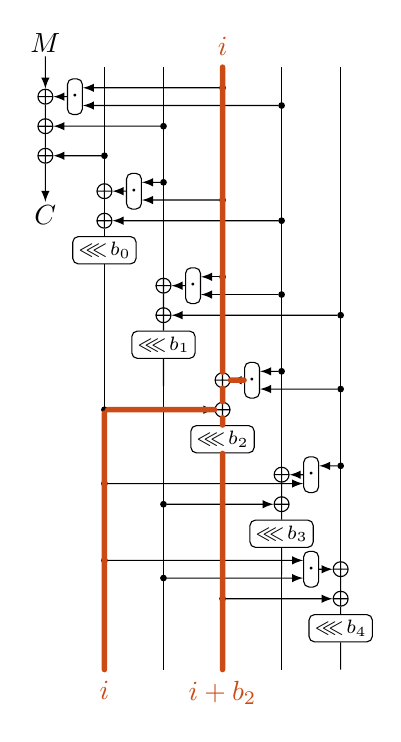
\begin{tikzpicture}[xscale=0.75,yscale=1.5]%{{{
    \printstate
    \draw[trail, epsil]
      (W-22) node[above] {$i$} -- (xnd2) (xnd2) -- (xor2) (xnd2) -- (and2)
      (xor2) -- (lll2) (xor2) -- (txor2) (txor2) -- (W40) node[below] {$i$}
      (lll2) -- (W42) node[below] {$i+b_2$}
      ;
  \end{tikzpicture}%}}}
  \caption*{$\varepsilon_i$: weight 1} %$S^{j,2}_i, S^{j+1,0}_i, S^{j+1,2}_{i+7}$ ($w\!=\!1$)}
  \end{subfigure}
  \hfill
  \begin{subfigure}{.32\textwidth}
    \small
    \begin{align*}
      \intertext{\cipher{MiniMORUS-640}:}
      \alpha_i:      && C_i &\to S^{0}_{i+5} \\
      \beta_i:       && C_i, S^0_i, S^1_i &\to 0 \\
      \gamma_i:      && S^1_i, S^4_i &\to S^1_{i+31} \\
      \delta_i:      && S^4_i &\to S^2_i, S^4_{i+13} \\
      \varepsilon_i: && S^2_i &\to S^0_i, S^2_{i+7}
      \intertext{\cipher{MiniMORUS-1280}:}
      \alpha_i:      && C_i &\to S^{0}_{i+13} \\
      \beta_i:       && C_i, S^0_i, S^1_i &\to 0 \\
      \gamma_i:      && S^1_i, S^4_i &\to S^1_{i+46} \\
      \delta_i:      && S^4_i &\to S^2_i, S^4_{i+4} \\
      \varepsilon_i: && S^2_i &\to S^0_i, S^2_{i+38}
    \end{align*}
    \caption*{\cipher{MiniMORUS} instances}
  \end{subfigure}
  \caption{\cipher{MiniMORUS} linear approximation fragments.}
  \label{fig:minimorus}
\end{figure}


\begin{figure}
  \newcommand{\M}[2]{1.65,-1.5*#1-.25-.25*#2}
  \newcommand{\C}[1]{-.1,-.25-1.5*#1}
  \renewcommand{\S}[2]{.25+.25*#2,-1.5*#1}
  \centering
  \begin{tikzpicture}[xscale=3, yscale=1.5, every node/.style={font=\scriptsize,inner sep=2pt}]
    \begin{scope}
      \foreach \r in {0,...,3} { \draw[gray, rounded corners=2pt] (0,-\r*1.5) rectangle ++(1.5,-1.5); }
      \foreach \r in {0,...,4} { \draw (\S{0}{\r}) node[above] {$S^{\r}$}; }
      \draw (\C{0}|-\S{0}{0}) node[above] {$C$};

      \draw[alpha] (\C{0}) node[left] {27} -| (\S{1}{0}) node[above right] {0}
                   (\M{0}{0}) node[right] {$\alpha_{27}$};

      \draw[beta]  (\C{1}) node[above left] {0} -| (\S{1}{0}) node[below right] {0}
                   (\C{1}-|\S{1}{0}) -| ([xshift=-1pt]\S{1}{1}) node[above] {0\,}
                   (\M{1}{0}) node[right] {$\beta_0$};
      \draw[alpha] ([yshift=-1.5pt]\C{1}) node[left] {8} -| (\S{2}{0}) node[above right] {\!\!13}
                   (\M{1}{1}) node[right] {$\alpha_{8,26}$};
      \draw[alpha] ([yshift=-3.0pt]\C{1}) node[below left] {26} -| ([xshift=-1pt]\S{2}{0}) node[above left] {31\!};
      \draw[gamma] (\S{1}{1}) node[above] {\,0} -- (\S{2}{1}) node[above left] {31\!\!}
                   (\S{1}{1}) ++(0,-.75) -| ([xshift=-1pt]\S{1}{4}) node[above] {0\,}
                   (\M{1}{2}) node[right] {$\gamma_0$};
      \draw[delta] (\S{1}{4}) node[above] {\,0} -- (\S{2}{4}) node[above right] {13}
                   (\S{1}{4}) ++(0,-1.25) -| ([xshift=2pt]\S{2}{2}) node[below] {0} node[black] {$\times$}
                   (\M{1}{3}) node[right] {$\delta_0$};

      \draw[beta]  (\C{2}) node[above left] {31} -| ([xshift=-1pt]\S{2}{0}) node[below left] {31\!}
                   ([xshift=-1pt]\C{2}-|\S{2}{0}) -| (\S{2}{1}) node[below left] {31\!\!}
                   (\M{2}{0}) node[right] {$\beta_{13,31}$};
      \draw[beta]  ([yshift=-1.5pt]\C{2}) node[left] {13} -| (\S{2}{0}) node[below right] {\!\!13}
                   ([yshift=-1.5pt]\C{2}-|\S{2}{0}) -| ([xshift=1pt]\S{2}{1}) node[above] {\,\,\,13};
      \draw[alpha] ([yshift=-3.0pt]\C{2}) node[below left] {7} -| (\S{3}{0}) node[above right] {12}
                   (\M{2}{1}) node[right] {$\alpha_7$};
      \draw[gamma] ([xshift=2pt]\S{2}{1}) node[below right] {13} -- ([xshift=2pt]\S{3}{1}) node[above right] {12}
                   ([xshift=2pt]\S{2}{1}) ++(0,-.75) -| (\S{2}{4}) node[below right] {13}
                   (\M{2}{2}) node[right] {$\gamma_{13}$};

      \draw[beta]  (\C{3}) node[left] {12} -| (\S{3}{0}) node[below right] {12}
                   (\C{3}-|\S{3}{0}) -| ([xshift=2pt]\S{3}{1}) node[below right] {12}
                   (\M{3}{0}) node[right] {$\beta_{12}$};

      \draw (\S{4}{2}) node[above] {\normalsize weight 7 (not 9)};
    \end{scope}

    \begin{scope}[xshift=2.5cm]
      \foreach \r in {1,...,4} { \draw[gray, rounded corners=2pt] (0,-\r*1.5) rectangle ++(1.5,-1.5); }
      \foreach \r in {0,...,4} { \draw (\S{1}{\r}) node[above] {$S^{\r}$}; }
      \draw (\C{0}|-\S{1}{0}) node[above] {$C$};

      \draw[alpha] (\C{1}) node[left] {2} -| (\S{2}{0}) node[above right] {7}
                   (\M{1}{0}) node[right] {$\alpha_{2}$};

      \draw[beta]  (\C{2}) node[above left] {7} -| (\S{2}{0}) node[below right] {7}
                   (\C{2}-|\S{2}{0}) -| ([xshift=-1pt]\S{2}{1}) node[above] {7\,}
                   (\M{2}{0}) node[right] {$\beta_7$};
      \draw[alpha] ([yshift=-1.5pt]\C{2}) node[left] {15} -| (\S{3}{0}) node[above right] {\!20}
                   (\M{2}{1}) node[right] {$\alpha_{15,1,27}$};
      \draw[alpha] ([yshift=-3.0pt]\C{2}) node[below left] {1} -| ([xshift=-1pt]\S{3}{0}) node[above left] {6\!};
      \draw[alpha] ([yshift=-4.5pt]\C{2}) node[below] {\,\,\,\,27} -| ([xshift=-3pt]\S{3}{0}) node[below] {0\,\,};
      \draw[gamma] (\S{2}{1}) node[above] {\,7} -- (\S{3}{1}) node[above left] {6\!}
                   (\S{2}{1}) ++(0,-.75) -| ([xshift=-1pt]\S{2}{4}) node[above] {7\,}
                   (\M{2}{2}) node[right] {$\gamma_7$};
      \draw[delta] (\S{2}{4}) node[above] {\,7} -- (\S{3}{4}) node[above right] {20}
                   (\S{2}{4}) ++(0,-1.25) -| ([xshift=1pt]\S{3}{2}) node[below] {\,7}
                   (\M{2}{4}) node[right] {$\delta_7$};
      \draw[epsil] (\S{2}{2}) node[above] {0} node[black] {$\times$} -- (\S{3}{2}) node[below] {7\,}
                   (\S{2}{2}) ++(0,-1.00) -| ([xshift=-4pt]\S{3}{0}) node[above left] {0}
                   (\M{2}{3}) node[right] {$\varepsilon_0$};

      \draw[beta]  (\C{3}) node[above left] {6} -| ([xshift=-1pt]\S{3}{0}) node[below left] {6\!}
                   ([xshift=-1pt]\C{3}-|\S{3}{0}) -| (\S{3}{1}) node[below left] {6\!}
                   (\M{3}{0}) node[right] {$\beta_{20,6}$};
      \draw[beta]  ([yshift=-1.5pt]\C{3}) node[left] {20} -| (\S{3}{0}) node[below right] {\!20}
                   ([yshift=-1.5pt]\C{3}-|\S{3}{0}) -| ([xshift=1pt]\S{3}{1}) node[above] {\,\,\,\,20};
      \draw[alpha] ([yshift=-3.0pt]\C{3}) node[below left] {14} -| (\S{4}{0}) node[above right] {19}
                   (\M{3}{1}) node[right] {$\alpha_{14}$};
      \draw[gamma] ([xshift=2pt]\S{3}{1}) node[below right] {20} -- ([xshift=2pt]\S{4}{1}) node[above right] {19}
                   ([xshift=2pt]\S{3}{1}) ++(0,-.75) -| (\S{3}{4}) node[below right] {20}
                   (\M{3}{2}) node[right] {$\gamma_{20}$};

      \draw[beta]  (\C{4}) node[left] {19} -| (\S{4}{0}) node[below right] {19}
                   (\C{4}-|\S{4}{0}) -| ([xshift=2pt]\S{4}{1}) node[below right] {19}
                   (\M{4}{0}) node[right] {$\beta_{19}$};

      \draw (\S{5}{2}) node[above] {\normalsize weight 9 (not 11)};
      \draw (\S{0}{2}) node[below] {\normalsize \cipher{MiniMORUS-640}};
    \end{scope}

    \draw[dashed] (\S{4.25}{-1}) -- (\S{4.25}{7}) -- ++(\S{1}{-1}) -- ++(\S{0}{7});

    \begin{scope}[yshift=-7.0cm]
      \foreach \r in {0,...,3} { \draw[gray, rounded corners=2pt] (0,-\r*1.5) rectangle ++(1.5,-1.5); }
      \foreach \r in {0,...,4} { \draw (\S{0}{\r}) node[above] {$S^{\r}$}; }
      \draw (\C{0}|-\S{0}{0}) node[above] {$C$};

      \draw[alpha] (\C{0}) node[left] {51} -| (\S{1}{0}) node[above right] {0}
                   (\M{0}{0}) node[right] {$\alpha_{51}$};

      \draw[beta]  (\C{1}) node[above left] {0} -| (\S{1}{0}) node[below right] {0}
                   (\C{1}-|\S{1}{0}) -| ([xshift=-1pt]\S{1}{1}) node[above] {0\,}
                   (\M{1}{0}) node[right] {$\beta_0$};
      \draw[alpha] ([yshift=-1.5pt]\C{1}) node[left] {55} -| (\S{2}{0}) node[above right] {\!4}
                   (\M{1}{1}) node[right] {$\alpha_{55,33}$};
      \draw[alpha] ([yshift=-3.0pt]\C{1}) node[below left] {33} -| ([xshift=-1pt]\S{2}{0}) node[above left] {46\!};
      \draw[gamma] (\S{1}{1}) node[above] {\,0} -- (\S{2}{1}) node[above left] {46\!}
                   (\S{1}{1}) ++(0,-.75) -| ([xshift=-1pt]\S{1}{4}) node[above] {0\,}
                   (\M{1}{2}) node[right] {$\gamma_0$};
      \draw[delta] (\S{1}{4}) node[above] {\,0} -- (\S{2}{4}) node[above right] {4}
                   (\S{1}{4}) ++(0,-1.25) -| ([xshift=2pt]\S{2}{2}) node[below] {0} node[black] {$\times$}
                   (\M{1}{3}) node[right] {$\delta_0$};

      \draw[beta]  (\C{2}) node[above left] {46} -| ([xshift=-1pt]\S{2}{0}) node[below left] {46\!}
                   ([xshift=-1pt]\C{2}-|\S{2}{0}) -| (\S{2}{1}) node[below left] {46\!}
                   (\M{2}{0}) node[right] {$\beta_{4,46}$};
      \draw[beta]  ([yshift=-1.5pt]\C{2}) node[left] {4} -| (\S{2}{0}) node[below right] {\!4}
                   ([yshift=-1.5pt]\C{2}-|\S{2}{0}) -| ([xshift=1pt]\S{2}{1}) node[above] {\,\,\,4};
      \draw[alpha] ([yshift=-3.0pt]\C{2}) node[below left] {37} -| (\S{3}{0}) node[above right] {50}
                   (\M{2}{1}) node[right] {$\alpha_{37}$};
      \draw[gamma] ([xshift=2pt]\S{2}{1}) node[below right] {4} -- ([xshift=2pt]\S{3}{1}) node[above right] {50}
                   ([xshift=2pt]\S{2}{1}) ++(0,-.75) -| (\S{2}{4}) node[below right] {4}
                   (\M{2}{2}) node[right] {$\gamma_{4}$};

      \draw[beta]  (\C{3}) node[left] {50} -| (\S{3}{0}) node[below right] {50}
                   (\C{3}-|\S{3}{0}) -| ([xshift=2pt]\S{3}{1}) node[below right] {50}
                   (\M{3}{0}) node[right] {$\beta_{50}$};

      \draw (\S{4}{2}) node[above] {\normalsize weight 7 (not 9)};
      \draw (\S{5}{2}) node[above] {\normalsize \cipher{MiniMORUS-1280}};
    \end{scope}

    \begin{scope}[xshift=2.5cm,yshift=-7.0cm]
      \foreach \r in {1,...,4} { \draw[gray, rounded corners=2pt] (0,-\r*1.5) rectangle ++(1.5,-1.5); }
      \foreach \r in {0,...,4} { \draw (\S{1}{\r}) node[above] {$S^{\r}$}; }
      \draw (\C{0}|-\S{1}{0}) node[above] {$C$};

      \draw[alpha] (\C{1}) node[left] {25} -| (\S{2}{0}) node[above right] {38}
                   (\M{1}{0}) node[right] {$\alpha_{25}$};

      \draw[beta]  (\C{2}) node[above left] {38} -| (\S{2}{0}) node[below right] {38}
                   (\C{2}-|\S{2}{0}) -| ([xshift=-1pt]\S{2}{1}) node[above] {38\,}
                   (\M{2}{0}) node[right] {$\beta_{38}$};
      \draw[alpha] ([yshift=-1.5pt]\C{2}) node[left] {7} -| (\S{3}{0}) node[above right] {\!20}
                   (\M{2}{1}) node[right] {$\alpha_{7,1,51}$};
      \draw[alpha] ([yshift=-3.0pt]\C{2}) node[below left] {29} -| ([xshift=-1pt]\S{3}{0}) node[above left] {42\!};
      \draw[alpha] ([yshift=-4.5pt]\C{2}) node[below] {\,\,\,\,51} -| ([xshift=-4pt]\S{3}{0}) node[below] {0\,\,\,};
      \draw[gamma] (\S{2}{1}) node[above right] {38} -- (\S{3}{1}) node[above left] {20\!}
                   (\S{2}{1}) ++(0,-.75) -| ([xshift=-1pt]\S{2}{4}) node[above left] {38}
                   (\M{2}{2}) node[right] {$\gamma_{38}$};
      \draw[delta] (\S{2}{4}) node[above] {\,38} -- (\S{3}{4}) node[above right] {42}
                   (\S{2}{4}) ++(0,-1.25) -| ([xshift=1pt]\S{3}{2}) node[below right] {38}
                   (\M{2}{4}) node[right] {$\delta_{38}$};
      \draw[epsil] (\S{2}{2}) node[above] {0} node[black] {$\times$} -- (\S{3}{2}) node[below] {38}
                   (\S{2}{2}) ++(0,-1.00) -| ([xshift=-5pt]\S{3}{0}) node[above left] {0}
                   (\M{2}{3}) node[right] {$\varepsilon_0$};

      \draw[beta]  (\C{3}) node[above left] {42} -| ([xshift=-1pt]\S{3}{0}) node[below left] {42\!}
                   ([xshift=-1pt]\C{3}-|\S{3}{0}) -| (\S{3}{1}) node[below left] {42\!}
                   (\M{3}{0}) node[right] {$\beta_{20,42}$};
      \draw[beta]  ([yshift=-1.5pt]\C{3}) node[left] {20} -| (\S{3}{0}) node[below right] {\!20}
                   ([yshift=-1.5pt]\C{3}-|\S{3}{0}) -| ([xshift=1pt]\S{3}{1}) node[above] {\,\,\,\,20};
      \draw[alpha] ([yshift=-3.0pt]\C{3}) node[below left] {11} -| (\S{4}{0}) node[above right] {24}
                   (\M{3}{1}) node[right] {$\alpha_{11}$};
      \draw[gamma] ([xshift=2pt]\S{3}{1}) node[below right] {42} -- ([xshift=2pt]\S{4}{1}) node[above right] {24}
                   ([xshift=2pt]\S{3}{1}) ++(0,-.75) -| (\S{3}{4}) node[below right] {42}
                   (\M{3}{2}) node[right] {$\gamma_{42}$};

      \draw[beta]  (\C{4}) node[left] {24} -| (\S{4}{0}) node[below right] {24}
                   (\C{4}-|\S{4}{0}) -| ([xshift=2pt]\S{4}{1}) node[below right] {24}
                   (\M{4}{0}) node[right] {$\beta_{24}$};

      \draw (\S{5}{2}) node[above] {\normalsize weight 9 (not 11)};
    \end{scope}
  \end{tikzpicture}
  \caption{\cipher{MiniMORUS}: Two approximations for $S^{2,2}_0$}
\end{figure}

\clearpage

\section{Linear Approximations for \cipher{MORUS}}

\end{document}
